\iffalse
Data used in this work include all subjects for whom baseline MRI data (T1-weighted MP-RAGE sequence at 1.5 T, typically 256 × 256 × 170 voxels with the voxel size of approximately 1 mm × 1 mm × 1.2 mm), at least moderately confident diagnoses (i.e. confidence > 2), hippocampus volumes (i.e. volumes of left and right hippocampi, calculated by FreeSurfer Version 4.3), and test scores in certain cognitive scales (i.e. ADAS: Alzheimer’s Disease Assessment Scale, range 0–85; CDR-SB: Clinical Dementia Rating ‘sum of boxes’, range 0–18; MMSE: Mini-Mental State Examination, range 0–30) were available.
Because one of the primary goals of our regression analysis is to identify a subset of imaging markers which are highly correlated to the AD progression reflected by the cognitive changes over time.
In summary, the identified longitudinally stable imaging markers are highly suggestive and strongly agree with the existing research findings,

The time points examined in this study for both imaging biomarkers and cognitive assessments include the baseline (BL), the 6th month (M6), the 12th month (M12), the 18th month (M18), the 24th month (M24) and the 36th month (M36).

As a result, a total of 544 sample subjects are selected in our study, among which 92 samples are diagnosed with AD, 205 samples are diagnosed to be with Mild Cognitive Impairment (MCI), and 177 samples are HC.

From the top panel of Fig. 4 we can see that the VBM biomarkers with highest weights are perfectly in accordance with existing medical findings. Specifically, we observe that the bilateral hippocampus are among the top selected biomarkers. In addition, the bilateral amygdala is also among the top selected biomarkers. Finally, We notice that the bilateral putamen are also among the top selected biomarkers. , which is one more indication of the correctness our new method.
Specifically, if the number of labeled images is small, semi-supervised approach appears to yield higher classification accuracy.
\fi

\section{Experiments} % 3.5 pages length recommended.
% The distribution of a feature may be categorized -> swap is better than gradient.
Our experiments consist of two parts; (1) we evaluate the prediction performance of the proposed model, and (2) we identify the biomarkers which are most important for AD progression prediction.
% We use AD progression in AD, MCI and HC as predictive targets in our studies.
% Although their deep learning approaches have shown the promising prediction results in binary classifications, but multi-class models have not achieved enough accuracy for clinical applicability.
\subsection{Competing Models and Hyperparameters}
We use the following hyperparameters found by the grid search. For our model, semi-supervised autoencoder (SAE), the static encoder $\phi_{SNP}$ and decoder $\psi_{SNP}$ has 2 fully connected layers (FC) each with the tanh activation function at the first to third layer and logistic sigmoid at the fourth layer. The dynamic decoder $\psi_{dynamic}$ has 3 FCs with activation function of leaky rectified linear unit (alpha = 0.1) at the first layer and tanh at the second and third layer. The dynamic encoder $\phi_{dynamic}$ is the LSTM with 64 units and tanh activation function. We set $\gamma_1 = 1e+2$, $\gamma_2 = 1e+1$, $\gamma_3 = 1$ in Eq.~\eqref{eq: total loss}.
To minimize the loss function in Eq.~\eqref{eq: total loss}, we adapt Adam optimizer~\cite{kingma2014adam} at a fixed learning rate of 0.0003 and the other parameters kept at their default values. We do not use any regularization or dropout technique, as they degrade the performance.

For an ablation study to observe the effectiveness of our semi-supervised enrichment learning, we introduce baseline LSTM (BLSTM) model as a competing model by removing decoders $\psi_{SNP}$ and $\psi_{dynamic}$ from our model SAE. In addition to the longitudinal model, we introduce the random forest~\cite{ho1995random} (RF) with 34 max depth and deep neural network (DNN) with 5 FCs as competing models. Since these baseline models are not longitudinal models, we provide the concatenation of most recent record $[\mathbf{x}_i^b, \mathbf{x}_i^s, \mathbf{x}_i^{n_i}]$ to them. Both the training and test set are provided to train SAE in a semi-supervised manner, while other competing models are trained only with the training set. Although the order of participants is randomly shuffled to avoid the bias, we use the same training and test data across all the competing methods for the fair comparison.
\subsection{Classification Performance}
We conduct the multiclass AD progression prediction task for 1 year ahead and evaluate the performance of the predictive models. We evaluate the predictive models with the following metrics:
\begin{equation}\label{eq: metrics}
\begin{aligned}
    &\text{Accuracy} = \frac{\sum_{c \in C}(TP_c + TN_c)}{\sum_{c \in C}(TP_c + TN_c + FP_c + FN_c)},\\
    &\text{Precision of class }c=\frac{TP_c}{TP_c + FP_c},\ \text{Recall of class }c=\frac{TP_c}{TP_c+FN_c},
\end{aligned}
\end{equation}
where $C$ is a set of classes \{AD, MCI, HC\}.
In table~\ref{tab: experimetal results}, the average and standard deviation of performance results across $k$ groups are reported following $k$-fold cross validation scheme. We split the dataset with $k=2,\ 3,\ 5$ subgroups, such that 50\%, 66\%, 80\% of participants belong to the training set respectively.
\begin{table*}[h]\label{tab: experimetal results}
    % \footnotesize
    %\scriptsize
    \small
    \setlength{\tabcolsep}{4pt} %% change column-wise separation.
    \centering
    \caption{The prediction results of SAE and the other competing models from $k$-fold cross validation. The best prediction is denoted as bold font.}\label{tab: prediction RMSE}
    \begin{tabular}{|c|c|c|c|c|c|} %% 6 columns table
    \hline
    {\bfseries $k$} & {\bfseries Metric} & \multicolumn{1}{c}{{\bfseries SAE} (Ours)} & \multicolumn{1}{c}{{\bfseries BLSTM}} & \multicolumn{1}{c}{{\bfseries RF}} & {\bfseries DNN}\\ %% Headers
    \Xhline{1pt}
    \multirow{7}{*}{5} %% 7 rows group.
    & Accuracy & \multicolumn{1}{c}{{\bfseries 74.95$\pm$4.72}} & \multicolumn{1}{c}{72.57$\pm$5.29} & \multicolumn{1}{c}{53.55$\pm$4.33} & 49.45$\pm$2.91\\
    & AD Precision & \multicolumn{1}{c}{{\bfseries 71.28$\pm$11.89}} & \multicolumn{1}{c}{71.19$\pm$16.79} & \multicolumn{1}{c}{51.55$\pm$5.22} & 55.13$\pm$6.30\\
    & MCI Precision & \multicolumn{1}{c}{59.84$\pm$10.11} & \multicolumn{1}{c}{{\bfseries 60.07$\pm$11.74}} & \multicolumn{1}{c}{nan$\pm$nan} & 33.84$\pm$4.97\\
    & HC Precision & \multicolumn{1}{c}{{\bfseries 89.69$\pm$7.33}} & \multicolumn{1}{c}{86.60$\pm$8.15} & \multicolumn{1}{c}{66.28$\pm$2.88} & 47.02$\pm$7.9\\
    & AD Recall & \multicolumn{1}{c}{69.30$\pm$7.30} & \multicolumn{1}{c}{65.92$\pm$21.31} & \multicolumn{1}{c}{{\bfseries 99.18$\pm$1.64}} & 74.49$\pm$7.45\\
    & MCI Recall & \multicolumn{1}{c}{{\bfseries 66.00$\pm$11.83}} & \multicolumn{1}{c}{60.00$\pm$8.57} & \multicolumn{1}{c}{0.47$\pm$0.93} & 22.89$\pm$2.93\\
    & HC Recall & \multicolumn{1}{c}{85.36$\pm$8.98} & \multicolumn{1}{c}{{\bfseries 89.37$\pm$6.53}} & \multicolumn{1}{c}{34.58$\pm$5.50} & 36.33$\pm$8.67\\
    \Xhline{1pt}
    \multirow{7}{*}{3} %% 7 rows group.
    & Accuracy & \multicolumn{1}{c}{{\bfseries 73.34$\pm$1.71}} & \multicolumn{1}{c}{69.92$\pm$1.94} & \multicolumn{1}{c}{53.83$\pm$1.02} & 47.81$\pm$1.65\\
    & AD Precision & \multicolumn{1}{c}{{\bfseries 63.47$\pm$7.84}} & \multicolumn{1}{c}{62.10$\pm$5.53} & \multicolumn{1}{c}{51.63$\pm$1.29} & 55.26$\pm$1.61\\
    & MCI Precision & \multicolumn{1}{c}{{\bfseries 63.97$\pm$8.74}} & \multicolumn{1}{c}{55.39$\pm$7.85} & \multicolumn{1}{c}{nan$\pm$nan} & 31.03$\pm$1.37\\
    & HC Precision & \multicolumn{1}{c}{{\bfseries 88.62$\pm$3.47}} & \multicolumn{1}{c}{85.94$\pm$3.09} & \multicolumn{1}{c}{65.74$\pm$3.14} & 46.64$\pm$6.77\\
    & AD Recall & \multicolumn{1}{c}{69.14$\pm$6.16} & \multicolumn{1}{c}{63.90$\pm$7.23} & \multicolumn{1}{c}{{\bfseries 98.48$\pm$0.8}} & 70.09$\pm$6.63\\
    & MCI Recall & \multicolumn{1}{c}{{\bfseries 56.97$\pm$8.32}} & \multicolumn{1}{c}{53.85$\pm$10.16} & \multicolumn{1}{c}{0.00$\pm$0.00} & 27.62$\pm$5.09\\
    & HC Recall & \multicolumn{1}{c}{{\bfseries 88.55$\pm$3.44}} & \multicolumn{1}{c}{85.48$\pm$3.04} & \multicolumn{1}{c}{36.56$\pm$2.84} & 32.44$\pm$6.52\\
    \Xhline{1pt}
    \multirow{7}{*}{2} %% 7 rows group.
    & Accuracy & \multicolumn{1}{c}{{\bfseries 72.29$\pm$2.44}} & \multicolumn{1}{c}{47.29$\pm$23.60} & \multicolumn{1}{c}{53.69$\pm$2.04} & 47.68$\pm$0.13\\
    & AD Precision & \multicolumn{1}{c}{{\bfseries 60.79$\pm$2.25}} & \multicolumn{1}{c}{50.38$\pm$26.69} & \multicolumn{1}{c}{51.56$\pm$2.68} & 52.87$\pm$2.26\\
    & MCI Precision & \multicolumn{1}{c}{{\bfseries 60.93$\pm$6.38}} & \multicolumn{1}{c}{nan$\pm$nan} & \multicolumn{1}{c}{nan$\pm$nan} & 33.12$\pm$6.56\\
    & HC Precision & \multicolumn{1}{c}{{\bfseries 86.99$\pm$2.20}} & \multicolumn{1}{c}{nan$\pm$nan} & \multicolumn{1}{c}{64.99$\pm$2.28} & 44.38$\pm$0.06\\
    & AD Recall & \multicolumn{1}{c}{72.90$\pm$8.45} & \multicolumn{1}{c}{81.36$\pm$18.64} & \multicolumn{1}{c}{{\bfseries 98.14$\pm$0.08}} & 75.56$\pm$5.73\\
    & MCI Recall & \multicolumn{1}{c}{{\bfseries 45.21$\pm$11.24}} & \multicolumn{1}{c}{30.19$\pm$30.18} & \multicolumn{1}{c}{0.53$\pm$0.53} & 20.51$\pm$2.42\\
    & HC Recall & \multicolumn{1}{c}{{\bfseries 89.85$\pm$4.13}} & \multicolumn{1}{c}{42.21$\pm$42.20} & \multicolumn{1}{c}{36.10$\pm$0.17} & 30.70$\pm$7.16\\
    % \Xhline{1pt}
    % \multirow{7}{*}{5} %% 7 rows group.
    % & Accuracy & \multicolumn{1}{c}{xx.xx$\pm$xx.xx} & \multicolumn{1}{c}{xx.xx$\pm$xx.xx} & \multicolumn{1}{c}{xx.xx$\pm$xx.xx} & xx.xx$\pm$xx.xx\\
    % & AD Precision & \multicolumn{1}{c}{xx.xx$\pm$xx.xx} & \multicolumn{1}{c}{xx.xx$\pm$xx.xx} & \multicolumn{1}{c}{xx.xx$\pm$xx.xx} & xx.xx$\pm$xx.xx\\
    % & MCI Precision & \multicolumn{1}{c}{xx.xx$\pm$xx.xx} & \multicolumn{1}{c}{xx.xx$\pm$xx.xx} & \multicolumn{1}{c}{xx.xx$\pm$xx.xx} & xx.xx$\pm$xx.xx\\
    % & HC Precision & \multicolumn{1}{c}{xx.xx$\pm$xx.xx} & \multicolumn{1}{c}{xx.xx$\pm$xx.xx} & \multicolumn{1}{c}{xx.xx$\pm$xx.xx} & xx.xx$\pm$xx.xx\\
    % & AD Recall & \multicolumn{1}{c}{xx.xx$\pm$xx.xx} & \multicolumn{1}{c}{xx.xx$\pm$xx.xx} & \multicolumn{1}{c}{xx.xx$\pm$xx.xx} & xx.xx$\pm$xx.xx\\
    % & MCI Recall & \multicolumn{1}{c}{xx.xx$\pm$xx.xx} & \multicolumn{1}{c}{xx.xx$\pm$xx.xx} & \multicolumn{1}{c}{xx.xx$\pm$xx.xx} & xx.xx$\pm$xx.xx\\
    % & HC Recall & \multicolumn{1}{c}{xx.xx$\pm$xx.xx} & \multicolumn{1}{c}{xx.xx$\pm$xx.xx} & \multicolumn{1}{c}{xx.xx$\pm$xx.xx} & xx.xx$\pm$xx.xx\\
    \cline{1-6}
    \end{tabular}
\end{table*}
In table~\ref{tab: experimetal results}, nan (not a number) indicates the denominator $TP_c + FP_c$ in Eq.~\eqref{eq: metrics} is zero, meaning the model never predicted class $c$. Considering the prediction of random forest is biased towards AD (high AD Recall), our model SAE generally outperforms other competing models. Interestingly, the performance gap between SAE and BLSTM increases as the size of training set decreases. We suppose that this is because our semi-supervised learning approach can learn from the unlabeled samples in test set, while BLSTM cannot. This finding shows the robustness of our model against number of unlabeled samples, as well as its promise in early diagnosis of AD.
% [Emphasize AD precision, recall as it is good, and important to detect than MCI and HC, can detect characteristics of the samples of AD participant.]
\subsection{AD Relevant Biomarkers Identification}
% [Because of the dramatic increase in the prevalence of AD, the identification of effective biomarkers for the early diagnosis and treatment of AD in individuals at high risk to develop the disease is crucial.]
It is vital to identify AD relevant biomarkers for early detection and treatment of AD in people at high risk of developing AD. Despite of the promising performance of deep neural networks, the predictions of deep neural networks are notoriously difficult to be interpreted. To identify which biomarkers (features) largely affect to the predictions, we add the perturbation to the input data and observe the changes in prediction.

For the longitudinal records of $q$-th biomarker ($1 \leq q \leq D_l$) and $i$-th participant, we sample the column vector of perturbations $\mathbf{p}_{i,q} \in \Re^{n_i}$ from the normal distribution $\mathcal{N}(0, \sigma_q^2)$ with zero mean and the same standard deviation as the observed distribution of $q$-th biomarker across all $n$ participants, and add the perturbation to the records as follows:
\begin{equation}
\begin{aligned}
    &N = \sum_{i=1}^n \sum_{j=1}^{n_i} \sum_{q=1}^{D_l} [\mathbf{M}_i]^j_q,\ \mu_q = \frac{1}{N}\sum_{i=1}^n \sum_{j=1}^{n_i} \sum_{q=1}^{D_l} [\mathbf{X}_i \odot \mathbf{M}_i]^j_q,\ \sigma_q^2 = \frac{1}{N}\sum_{i=1}^n \sum_{j=1}^{n_i} \sum_{q=1}^{D_l}\\
    &[\mathbf{M}_i]^j_q ([\mathbf{X}_i]^j_q - \mu_q)^2,\ \mathbf{X}_i' = [[\mathbf{X}_i]_1, [\mathbf{X}_i]_2, \cdots, [\mathbf{X}_i]_q + \mathbf{p}_{i, q}, \cdots, [\mathbf{X}_i]_{D_l}].
\end{aligned}
\end{equation}
Then the prediction changes by the perturbation is:
\begin{equation}\label{eq: neuroimaging identification}
\begin{aligned}
    &\Delta\tilde{\mathbf{y}}_i = \| \psi_{pred}\bigl(\phi_{dynamic}(\mathbf{X}_i', \mathbf{M}_i, \mathbf{t}_i;\ \theta_{\phi}^l),\ \psi_{SNP}(\phi_{SNP}(\mathbf{x}_i^s;\ \theta^s_{\phi});\ \theta^s_{\psi}),\ \mathbf{x}_i^b;\ \theta^p_{\psi}\bigr)\\
    &- \psi_{pred}\bigl(\phi_{dynamic}(\mathbf{X}_i, \mathbf{M}_i, \mathbf{t}_i;\ \theta_{\phi}^l),\ \psi_{SNP}(\phi_{SNP}(\mathbf{x}_i^s;\ \theta^s_{\phi});\ \theta^s_{\psi}),\ \mathbf{x}_i^b;\ \theta^p_{\psi}\bigr)\|_1.
\end{aligned}
\end{equation}
The importance of $q$-th biomarker is the average of prediction changes across all the participants: $\frac{1}{n}\sum_{i=1}^n\Delta\tilde{\mathbf{y}}_i$. Similarly, we can calculate the input genetic data whose $q$-th SNP is perturbed and it's prediction changes.
% \begin{equation}\label{eq: SNPs identification}
% \begin{aligned}
%     &(\mathbf{x}_i^s)' = [x_{i, 1}^s, x_{i, 2}^s, \cdots, x_{i, m}^s + p_{i, m}, \cdots, x_{i, D_s}^s],\\
%     &\Delta\tilde{\mathbf{y}}_i = \| \psi_{pred}\bigl(\phi_{dynamic}(\mathbf{X}_i, \mathbf{M}_i, \mathbf{t}_i;\ \theta_{\phi}^d),\ \psi_{SNP}(\phi_{SNP}((\mathbf{x}_i^s)';\ \theta^s_{\phi});\ \theta^s_{\psi}),\ \mathbf{x}_i^b;\ \theta^p_{\psi}\bigr)\\
%     &- \psi_{pred}\bigl(\phi_{dynamic}(\mathbf{X}_i, \mathbf{M}_i, \mathbf{t}_i;\ \theta_{\phi}^d),\ \psi_{SNP}(\phi_{SNP}(\mathbf{x}_i^s;\ \theta^s_{\phi});\ \theta^s_{\psi}),\ \mathbf{x}_i^b;\ \theta^p_{\psi}\bigr)\|_1.
% \end{aligned}
% \end{equation}
% Finally, we plot top 15 most important features in Fig..
\subsubsection{Identifying AD relevant imaging biomarkers}
\begin{figure}
    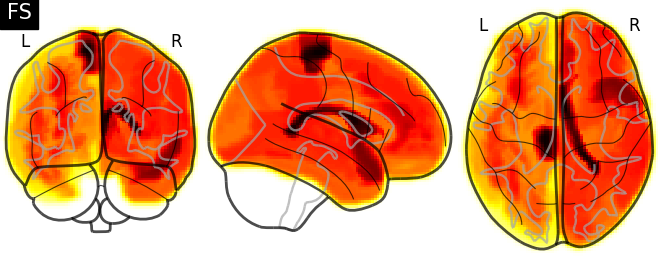
\includegraphics[width=0.49\textwidth]{images/biomarker-identification/fs.png}
    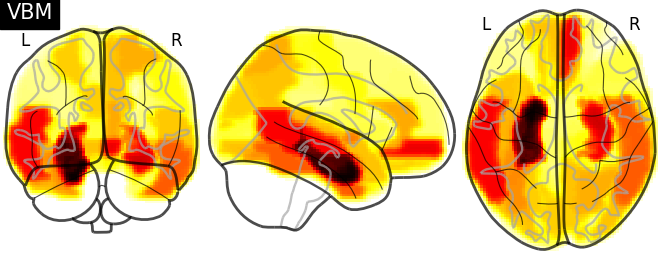
\includegraphics[width=0.49\textwidth]{images/biomarker-identification/vbm.png}
    \caption{Importance distribution over the brain regions. The darker color indicates the larger importance. The top five most important regions identified are {\bf FS:} Right Lateral Ventricle, Left Para-Hippocampal, Left Amygdala, Left Cerebral White Matter, Left Hippocampus, and {\bf VBM:} Left Para-Hippocampal, Left Amygdala, Left Hippocampus, Right Hippocampus, Right Amygdala.}
    \label{fig: brain map}
\end{figure}
\begin{figure}
    \centering
    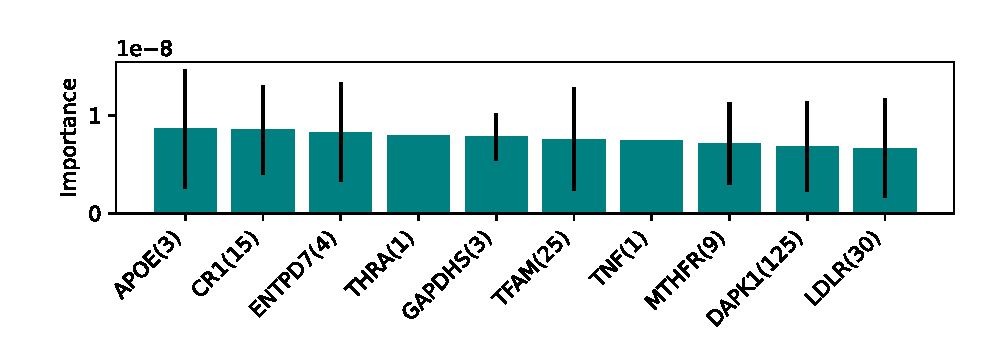
\includegraphics[width=0.9\textwidth]{images/biomarker-identification/alzgene-same-color.eps}
    \caption{Importance of each AlzGene group. The standard deviation and number of SNPs of each group is denoted by the line length at the head of each bar and the number next to the group name respectively.}\label{fig: AlzGene}
\end{figure}
In Fig~\ref{fig: brain map}, we plot the importance distribution over the brain regions calculated by Eq.~\eqref{eq: neuroimaging identification}. The identified regions have been shown in the literature to be related to AD. For example, the previous studies~\cite{carmichael2007ventricular} found that ventricular volume and its rate of change is related with vulnerability to cognitive decline and dementia. 
% \cite{carmichael2007ventricular,jack2004comparison}
They observe that the larger ventricles in healthy participants increase the probability to the progression of dementia-related disease in the future. The hippocampus is vulnerable to be damaged from AD~\cite{mu2011adult} and has been shown to affect long-term memory and spatial navigation in patients with AD. Finally, the amygdala region, also identified by our approach, is also severely affected by AD~\cite{poulin2011amygdala} and is associated with emotional response and decision-making.
\subsubsection{Identifying AD relevant genetic biomarkers}
We plot the importance distribution over the AlzGene groups of SNPs in Fig~\ref{fig: AlzGene}. The AlzGene groups of SNPs have been constructed by the multiple genome-wide association studies listed on the website (\url{http://www.alzgene.org/}). Apolipoprotein E (APOE) group is identified by our approach, and APOE genes involve in amyloid beta peptide (A$\beta$) aggregation and clearance~\cite{kim2009role}. The accumulation of A$\beta$ is commonly observed in the progress of AD~\cite{chen2017amyloid} and amyloid hypothesis suggests reasonable mechanism how the accumulation of A$\beta$ can result neuronal malfunction~\cite{hardy2002amyloid}. In addition, $\epsilon$4 allele of APOE gene increase risk factor for AD and decrease the age of AD onset~\cite{corder1993gene}. For complement receptor 1 (CR1) group, genome-wide analysis~\cite{lambert2009genome} reported CR1 association with late-onset AD. The subset of biomarkers identified in the FreeSurfer, VBM, and SNP modalities, provides the substantial evidence that our approach can identify the biomarkers associated with AD.
% [Why multi-class classification? -> the different clinical actions are required for stage : AD, MCI, HC]
% even if very few samples are labeled.